%!TEX root = ../../../main.tex
\section{Navigation Controller} % (fold)
\label{sec:mr_navigation_controller}
Using the processed information from the sensors and the different kind of navigations, the robot is able to move and satisfy all the requirements from the project.
In this section the \emph{navigation controller} is explained.
This is in charge of find the path, and actions associated to that path, given two nodes.

\subsection{Navigation state representation} % (fold)
    \label{sub:mr_navigation_state_representation}
    In order to navigate from one position to the desired one, a graph of the possible states in which the robot is stopped or idle has been represented.
    This graph depicts all the possible states of the mobile robot in which the robot has not movement along with their associated transference functions. 
    These are other states in which the robot is moving or changing its state and in this project are called \emph{skills} (Section \ref{sub:skills}).
    In the figure \ref{fig:mr_graph} the graph of the project is shown.
    
    As an example, in the transference between the node \emph{"Workcell Exit"} and \emph{"Line End"}, the associated conditions are shown. 
    These are: first, needs to \emph{turn 90 degrees clockwise}, then \emph{follow the line until the QR "line\_out"} is detected, all this done with the collision detector turned on and changing the internal position of the robot in the end.

    \begin{figure}[ht!]
        \centering
        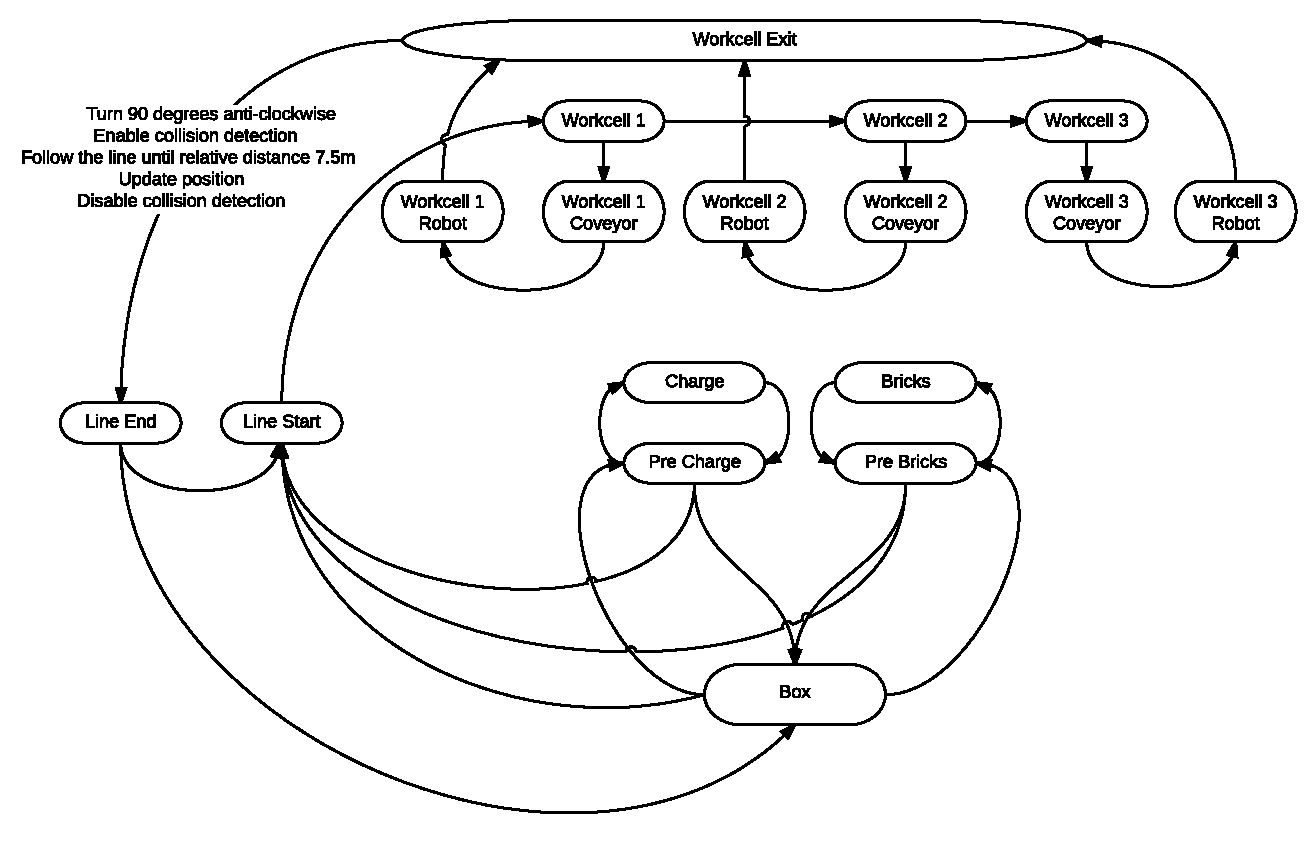
\includegraphics[width=\textwidth]{figs/mr_graph.pdf}
        \caption{Graph representation adopted in the project}
        \label{fig:mr_graph}
    \end{figure}

    % subsection navigation_state_representation (end)

    \subsection{Skills} % (fold)
    \label{sub:skills}
    As stated before, the skills are states of the robot in which this is changes its physical condition.
    They let the robot change its state and position.
    The implementation is based on a couple between one of the navigation types and some information from the sensors used as a condition.
    The skills designed and implemented are:
    \begin{itemize}
        \item Follow the line until desired QR
        \item Follow the line until desired LIDAR distance
        \item Follow the line until desired relative distance
        \item Linear move
        \item Angular move
        \item Go to free position
        \item Detect obstacles
        \item Wait
    \end{itemize}
    % subsection skills (end)

    \subsection{Artificial intelligence} % (fold)
    \label{sub:mr_artificial_intelligence}
    So as to find the most optimal path between two nodes in the graph an artificial intelligence (AI) has been designed and implemented.
    All the transferences between states have an associated cost which is used by a Breadth First Search (BFS).

    The BFS is an algorithm of searching for graphs that explores all the neighbors of the root, then the neighbors of this ones etc.
    Is a complete search algorithm and optimal meaning that will always find the optimal solution.
    In this case as the cost between nodes is the distance, the BFS will always find the shortest path.
    
    The negative part of the BFS is the space complexity but, as a result of the small graph, the search time is in the order of milliseconds.
    % subsection artificial_intelligence (end)
% section navigation_controller (end)
